 % !TeX spellcheck = en_US
\documentclass[french]{yLectureNote}

\title{Optique Géométrique}
\subtitle{Niveau 1}
\author{Paulhenry Saux}
\date{\today}
\yLanguage{Français}

\professor{C.Gatel}%christophe.gatel@cemes.fr : section B sillon 7

\usepackage{graphicx}%----pour mettre des images
\usepackage[utf8]{inputenc}%---encodage
\usepackage{geometry}%---pour modifier les tailles et mettre a4paper
%\usepackage{awesomebox}%---pour les boites d'exercices, de pbq et de croquis ---d\'esactiv\'e pour les TP de PC
\usepackage{tikz}%---pour deiffner + d\'ependance de chemfig
\usepackage{tkz-tab}
\usepackage{chemfig}%---pour deiffner formules chimiques
\usepackage{chemformula}%---pour les formules chimiques en \'equation : \ch{...}
\usepackage{tabularx}%---pour dimensionner automatiquement les tableaux avec variable X
\usepackage{awesomebox}%---Pour les boites info, danger et autres
\usepackage{menukeys}%---Pour deiffner les touches de Calculatrice
\usepackage{fancyhdr}%---pour les en-t\^ete personnalis\'ees
\usepackage{blindtext}%---pour les liens
\usepackage{hyperref}%---pour les liens (\`a mettre en dernier)
\usepackage{caption}%---pour la francisation de la l\'egende table vers Tableau
\usepackage{pifont}
\usepackage{array}%---pour les tableaux
\usepackage{lipsum}
\usepackage{yFlatTable}
\usepackage{multicol}
\newcommand{\Lim}[1]{\lim\limits_{\substack{#1}}\:}
\renewcommand{\vec}{\overrightarrow}
\begin{document}
%\titleOne
\setcounter{chapter}{3}
\chapter{Dioptres sphériques dans l'approximation de Gauss}
\section{Définitions}
\begin{definition}[Dioptre sphérique]
C'est un dioptre avec une symétrique axiale. Quand la courbure de la sphère est avant le dioptre, c'est un diptre concave. Dans l'autre cas, c'est un dioptre convexe.
\end{definition}
L'axe optique passe par le centre $C$ de l'axe optique. $S$ est l'intesection entre l'axe optique et le sommet du dioptre. Il est réel, contrairement à $C$.

Un dioptre concave a une distance $\bar{SC} < 0$.

Un dioptre convexe a une distance $\bar{SC} > 0$.

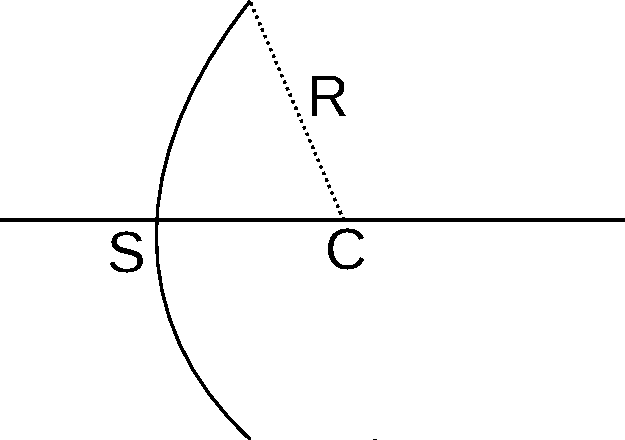
\includegraphics[scale=0.5]{dioptre_convexe}
\criticalInfo{Vergence d'un dioptre}{La concavité d'un dioptre ne détermine pas entièrement la vergence ! Il faut aussi prendre en compte l'indice des milieux}

\section{Stigatisme du dioptre sphérique}
\begin{theorem}[Loi des sinus]
 Le rapport du c\^oté opposé à l'angle sur l'angle est constant dans tout le triangle.
\end{theorem}
% Dans $CIA_o : \frac{\bar{CA_o}}{\sin i_1} = \frac{\bar{IA_o}}{\sin\omega}$
%
% Dans $CIA_i : \frac{\bar{CA_i}}{\sin i_2} = \frac{\bar{IA_i}}{\sin\omega}$
%
% On obtient : $n_o\frac{\bar{CA_o}}{\bar{IA_o}} = n_i \frac{\bar{CA_i}}{\bar{IA_i}}$
%
% En se plaçant dans les conditions de Gauss, on a $\bar{IA_o} \sim \bar{SA_o}$ et $\bar{IA_i} \sim \bar{SA_i}$.
%
% On obtient la relation de conjugaison de Descartes

\begin{theorem}[Relation de conjugaison de Descartes]
 Dans les conditions de Gauss, on a \[ \frac{n_i}{\bar{SA_i}} - \frac{n_o}{\bar{SA_o}} = \frac{n_i-n_o}{\bar{SC}} = \text{ Vergence }\] avec \(A_i\) le point image et \(A_o\) le point objet
\end{theorem}
\warningInfo{Vergence}{Si \(V>0\), le dioptre est convergent. Dans le cas contraire, il est divergent. Le caractère de convergence est défini par rapport à des rayons à l'infini}
\section{Foyers du dioptre sphérique}
\begin{definition}[Foyers images/objet]
Le foyer image est l'emplacement du conjugué d'un objet à l'infini. Le foyer objet est l'emplacement du conjugué d'une image à l'infini.
\end{definition}
% Quand $A_o \to \infty, A_i \to F_i \Rightarrow \bar{SA_o} \to \infty, \bar{SA_i} \to \bar{SF_i}$ et $\frac{n_i}{\bar{SF_i}} = \frac{n_i-n_o}{\bar{SC}}$.
%
% On appelle $\bar{SF_i} = \frac{n_i}{V}$ la distance focale image. Quand la focale est négative, le système est divergent.
\subsection{Distances focales}
\begin{definition}
La focale (image) est \(\bar{SF_i} = \frac{n_i}{V}\) et la focale objet est  \(\bar{SF_0} =- \frac{n_o}{V}\). les 2 sont liés par \(\frac{\bar{SF_i}}{\bar{SF_o}} = \frac{-n_i}{n_0}\)
\end{definition}
% La focale (image) est \(\bar{SF_i} = \frac{n_i}{V}\) et la focale objet est  \(\bar{SF_0} =- \frac{n_o}{V}\).
%
% Pour les obtenir, on utilise les relations de Descartes en se plaçant à l'infini dans certains cas.
%
% Les 2 sont liées : \(\frac{\bar{SF_i}}{\bar{SF_o}} = \frac{-n_i}{n_0}\).
\subsection{Position du foyer}
Si un dioptre est convergent, \(\bar{SF_i} > 0 \Rightarrow\) le foyer image est après S,  \(\bar{SF_i} < 0 \Rightarrow\) il est avant S.

Si un dioptre est divergent, \(\bar{SF_i} < 0 \Rightarrow\) il est après S,  \(\bar{SF_i} > 0 \Rightarrow\) il est avant S.\marginInfo{Lorsque la vergence augmente, la distance focale diminue. Un système à petite focale a une grande vergence.}

% Le conjugué de $C$ est lui-m\^eme.
\section{Grandissement transversal}
\begin{definition}
\[G_t = \frac{\bar{A_iB_i}}{\bar{A_oB_o}} = \frac{\bar{CA_i}}{\bar{CA_o}} = \frac{n_0\bar{SA_i}}{n_1\bar{SA_o}}\]
\end{definition}
Une image est renversée quand $G_t$ est négatif.

Une image est droite quand $G_t$ est positif.

% Pour augmenter le grandissement, on doit rapprocher le point objet du système.
\section{Construction}
\warningInfo{Règles de constrcution}{
\begin{itemize}
 \item Tout rayon (émergent ou incident) passant par \(c\) n'est pas dévié.
 \item Tout rayon incident parallèement à l'axe optique passe par le foyer image \(F_i\)
  \item Tout rayon incident passant par \(F_o\) émerge parralèlement à l'axe optique.
  \item On respecte la convention traits plains/pointillés : les rayons pleins existent vraiment.
\end{itemize}
}
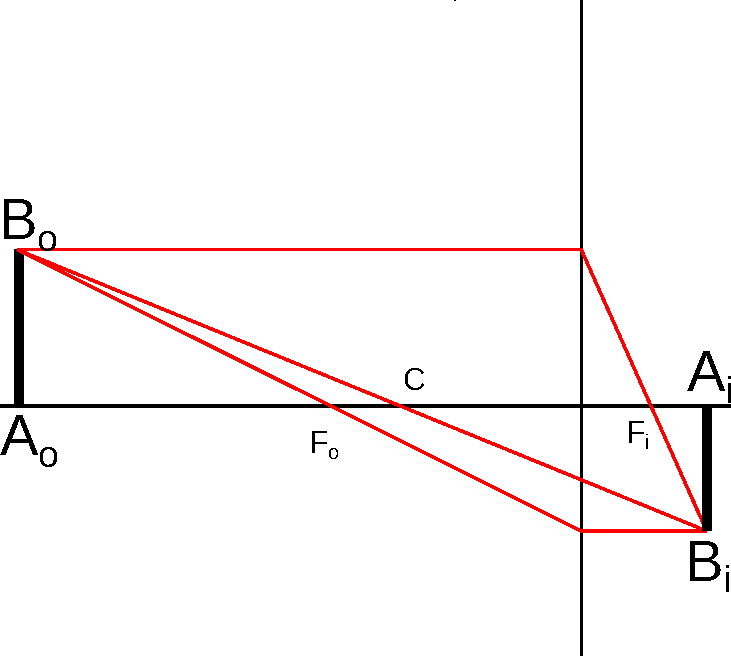
\includegraphics[scale=0.3]{c4-2} 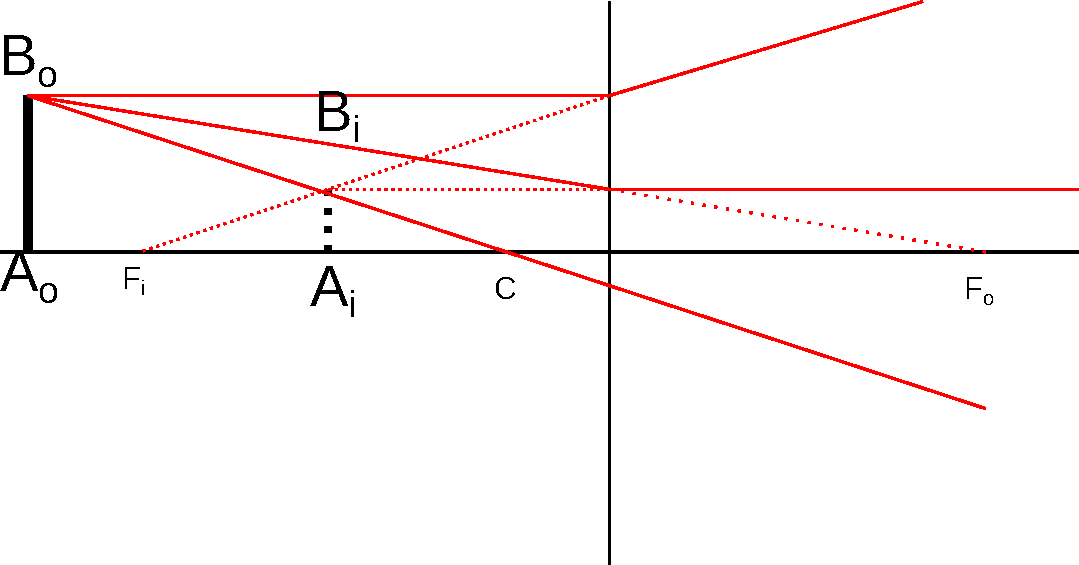
\includegraphics[scale=0.3]{c4-3}
% On trace d'abord le rayon non dévié passant pas C
%
% On trace ensuite le rayon parallèle à l'axe optique.
%
% $SA_i >0$ et $SA_o <0$, donc image renversée.
\section{Étude de dioptres plans}
\warningInfo{Caractérisation}{La vergence d'un dioptre plan est nulle, on a  donc la relation ; \[\frac{n_i}{\bar{SA_i}} = \frac{n_o}{\bar{SA_{o}}}\]}
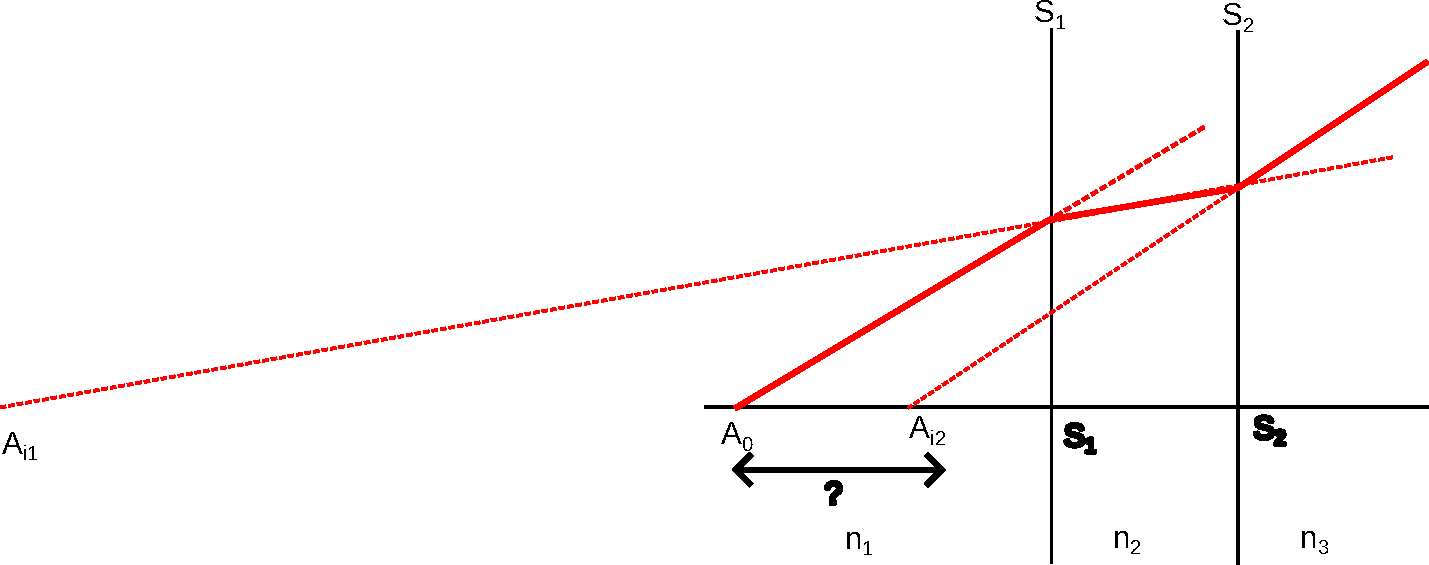
\includegraphics[scale=0.5]{path1}

On étudie 2 dioptres plans placés les uns à la suite des autres, avec 3 indices de milieu différent. On a $n_2>n_1>n_3$ et on cherche l'écart entre l'image d'un objet et l'objet en question.

Il y a 2 dioptres dans lesquels on peut écrire la relation de conjugaison :
\[\frac{n_1}{\bar{S_1A_0}} = \frac{n_2}{\bar{S_1A_{i1}}} \text{ et } \frac{n_2}{\bar{S_2A_{0,2}}} = \frac{n_3}{\bar{S_2A_{i2}}}\]

Or, l'image du premier dioptre est l'objet du second dioptre. On peut donc écrire $S_2A_{0,2} = \bar{S_2S_1} + \bar{S_1A_{i1}}$ en utilisant la relation Chasles.\marginCritical{On ne peut pas écrire directement $S_2A_{0,2} = \bar{S_1A_{i1}}$ car bien que les points images et objet soient les m\^emes, la distance ne l'est pas car l'une dépend de $S_1$ et l'autre de $S_2$.}

En se servant des relations de conjugaison, on trouve $\bar{S_1A_{i1}}$ que l'on injecte après transformation dans la relation du deuxième dioptre pour trouver $S_2A_{i2}$

La différence recherchée vaut finalement $\bar{A_0A_{i2}} = \bar{A_0S_1} + \bar{S_1S_2} + \bar{S_2A_{i2}}$ par la relation de Chasles, en connaissant la distance à laquelle se trouve l'objet, l'indice des milieux et la distance entre les 2 dioptres.
\end{document}

